\documentclass[runningheads]{llncs}
\usepackage[T1]{fontenc}
\usepackage[utf8]{inputenc}
\usepackage[spanish]{babel}
\usepackage{graphicx}
\usepackage{amsmath}
\usepackage{array}
\usepackage{hyperref}

\begin{document}

\title{Taller de Fotografía Forense Digital: análisis de falla de una palanqueta de acero}

\author{Sara Kemelmajer \and Rocío Ana Martinez \and María Pilar Mujica \and Lucía Salamone}

\authorrunning{S. Kemelmajer et al.}

\institute{Universidad Nacional de Cuyo, Instituto de Ingeniería Industrial\\
\url{https://ingenieria.uncuyo.edu.ar/}}

\maketitle

\begin{abstract}
El presente informe documenta el trabajo realizado en el taller de fotografía forense digital, cuyo objetivo fue registrar de forma objetiva y reproducible una pieza metálica deteriorada y, a partir de ese registro, determinar la causa más probable de su falla. La pieza analizada es una palanqueta de acero que presenta deformación permanente y oxidación superficial. Se aplicó un protocolo fotográfico que va de lo general a lo particular y se interpretaron las evidencias visibles. Se concluye que la herramienta falló por sobrecarga mecánica estática de flexión, originada en un uso inadecuado, descartándose la fatiga, los defectos de fabricación y la fractura frágil. Finalmente, se proponen mejoras al protocolo fotográfico y ensayos complementarios para un peritaje completo.

\keywords{UNCUYO \and Fotografía forense \and Análisis de fallas \and Deformación plástica \and Flexión.}
\end{abstract}

\section{Introducción y objetivo}

El taller tuvo como objetivo aplicar las técnicas de fotografía forense digital para documentar, de forma objetiva y reproducible, una pieza metálica deteriorada y, a partir de ese registro, determinar la causa más probable de su falla. La inspección se realizó el 18 de septiembre de 2026.

Los objetivos específicos fueron:

\begin{enumerate}
\item Fijar fotográficamente el estado de la pieza tal como fue recibida, antes de cualquier manipulación o ensayo.
\item Documentar la geometría general y los detalles (extremos, curvaturas, superficie) con un protocolo de tomas ordenado.
\item Interpretar las evidencias visibles para identificar el mecanismo de falla.
\item Elaborar un informe técnico que pueda ser revisado por terceros sin necesidad de acceder a la pieza física.
\end{enumerate}

\section{Fundamentos: ¿por qué se toman fotografías en una pericia?}

La fotografía forense es el primer paso de cualquier análisis de falla: congela el estado de la evidencia en el momento en que se recibe. Una vez que la pieza se limpia, se corta o se ensaya, ese estado se pierde para siempre \cite{astm860,asm11}. Sus funciones principales son:

\begin{itemize}
\item \textbf{Preservar la evidencia:} deja un registro permanente aunque la pieza se pierda, se altere o se destruya en ensayos posteriores.
\item \textbf{Garantizar objetividad:} la imagen muestra lo que hay, sin depender de la interpretación de quien inspecciona.
\item \textbf{Permitir el análisis posterior:} se pueden revisar detalles y comparar zonas sin manipular la pieza.
\item \textbf{Sostener las conclusiones:} cada afirmación del informe se respalda con una fotografía verificable.
\item \textbf{Comunicar a terceros:} peritos, docentes, jueces o clientes comprenden el caso sin estar presentes.
\item \textbf{Mantener la cadena de custodia:} las fotografías fechadas y numeradas acreditan que la pieza analizada es la misma que se recibió.
\end{itemize}

En la ingeniería, la misma lógica se aplica en mantenimiento, control de calidad y análisis de fallas industriales: documentar antes de intervenir permite encontrar la causa raíz y evitar que el problema se repita.

\section{Metodología y protocolo fotográfico}

Se siguió el criterio de la fotografía forense de ir \emph{de lo general a lo particular}: primero se registra la pieza completa y luego los detalles relevantes.

\begin{enumerate}
\item \textbf{Recepción e identificación:} la pieza se fotografió tal como fue recibida, sin limpiarla ni modificarla.
\item \textbf{Fondo neutro:} se utilizó una mesa blanca y lisa para dar contraste con el acero oscuro y facilitar la lectura del contorno.
\item \textbf{Vistas generales:} tomas de perfil y longitudinales completas para mostrar la geometría y la curvatura global.
\item \textbf{Vistas de detalle:} acercamientos a los extremos, a la sección transversal y a las zonas con marcas o corrosión.
\item \textbf{Vistas complementarias:} vista posterior para evaluar la alineación del eje desde otro plano.
\item \textbf{Registro y numeración:} cada fotografía se numeró y describió para vincularla al análisis.
\end{enumerate}

El equipo utilizado fue la cámara digital de un teléfono celular, con iluminación ambiente del aula-taller.

\section{Objeto de estudio}

La pieza es una herramienta manual de acero conocida como palanqueta o barra de fuerza/desencofrado, utilizada para hacer palanca, separar elementos o desclavar. Sus características se resumen en la Tabla~\ref{tab:pieza}.

\begin{table}
\caption{Características observadas de la pieza.}\label{tab:pieza}
\centering
\begin{tabular}{|p{3.2cm}|p{7.5cm}|}
\hline
\textbf{Característica} & \textbf{Observación}\\
\hline
Material & Acero al carbono (presunto, por aspecto y uso)\\
Sección & Aproximadamente circular/hexagonal\\
Extremo superior & Plano, con bisel tipo cincel\\
Extremo inferior & Curvado, en forma de gancho o pata\\
Estado general & Curvatura fuera de diseño, marcas de golpes y óxido superficial\\
Dimensiones & No se registró escala en las fotografías (ver Sección~\ref{sec:limitaciones})\\
\hline
\end{tabular}
\end{table}

\section{Descripción del deterioro y análisis de causas}

La inspección visual identificó tres tipos de daño. El principal es una deformación plástica por flexión; los otros dos son secundarios.

\subsection{Deformación plástica permanente (flexión)}

La barra presenta una curvatura pronunciada que no corresponde a su geometría original (Fig.~\ref{fig:general}). Que la deformación sea permanente indica que el esfuerzo aplicado superó el límite elástico del material ($\sigma_y$) y el acero ingresó en la zona plástica: al retirar la carga, la pieza no recuperó su forma \cite{callister}.

En una barra utilizada como palanca, la tensión máxima de flexión se calcula como \cite{beer}:

\begin{equation}
\sigma_{max} = \frac{M \cdot c}{I} = \frac{F \cdot L \cdot c}{I}
\label{eq:flexion}
\end{equation}

donde $F$ es la fuerza aplicada en el mango, $L$ el brazo de palanca, $c$ la distancia desde el eje neutro hasta la fibra más alejada e $I$ el momento de inercia de la sección. La deformación permanente aparece cuando $\sigma_{max} > \sigma_y$. La Ec.~(\ref{eq:flexion}) explica por qué alargar el brazo de palanca (por ejemplo, con un caño) multiplica el riesgo: el momento crece en proporción directa a $L$.

\subsection{Origen del esfuerzo}

El perfil curvado y la distorsión de los extremos indican que la herramienta se utilizó como palanca con cargas de flexión excesivas. Lo más probable es que se haya forzado un punto de alta resistencia o se haya excedido el brazo de palanca recomendado. Las marcas de golpes cerca del extremo superior (Fig.~\ref{fig:detalle}) sugieren, además, su uso como elemento de impacto.

\subsection{Deterioro superficial (oxidación)}

Se observan texturas rugosas y zonas de corrosión atmosférica (óxido de hierro hidratado), producto de la exposición ambiental y del desgaste del recubrimiento original. Se trata de una corrosión superficial y uniforme: no se aprecian picaduras profundas ni pérdida de sección significativa, por lo que no compromete la integridad interna de la pieza.

\subsection{Mecanismos descartados}

La Tabla~\ref{tab:descartados} resume los mecanismos de falla evaluados y el fundamento por el cual se descartan \cite{asm11}.

\begin{table}
\caption{Mecanismos de falla descartados.}\label{tab:descartados}
\centering
\begin{tabular}{|p{3.4cm}|p{7.3cm}|}
\hline
\textbf{Mecanismo} & \textbf{Fundamento del descarte}\\
\hline
Fatiga cíclica & No hay fisuras ni marcas de playa; la pieza está deformada, no fracturada\\
Defecto de fabricación & No se observan inclusiones, porosidades ni discontinuidades superficiales\\
Fractura frágil & La pieza se dobló sin romperse, comportamiento típico de un material dúctil\\
Corrosión como causa principal & La oxidación es superficial y no redujo la sección resistente\\
\hline
\end{tabular}
\end{table}

\section{Registro fotográfico forense}

Se tomaron cinco fotografías, ordenadas de lo general al detalle. La Tabla~\ref{tab:fotos} indica qué evidencia documenta cada una.

\begin{table}
\caption{Registro de fotografías.}\label{tab:fotos}
\centering
\begin{tabular}{|p{1.4cm}|p{3.6cm}|p{5.7cm}|}
\hline
\textbf{N.º} & \textbf{Vista} & \textbf{Evidencia documentada}\\
\hline
Foto 1 & Perfil general & Curvatura global y extremo en gancho deformado\\
Foto 2 & Detalle del extremo superior & Marcas de golpes, corrosión y desvío del eje\\
Foto 3 & Sección transversal superior & Forma de la sección y curvatura cerca del extremo\\
Foto 4 & Longitudinal completa & Perfil completo y comparación entre extremos\\
Foto 5 & Posterior / alineación & Falta de rectitud vista desde otro plano\\
\hline
\end{tabular}
\end{table}

\begin{figure}
\centering
\begin{minipage}[b]{0.45\textwidth}
\centering
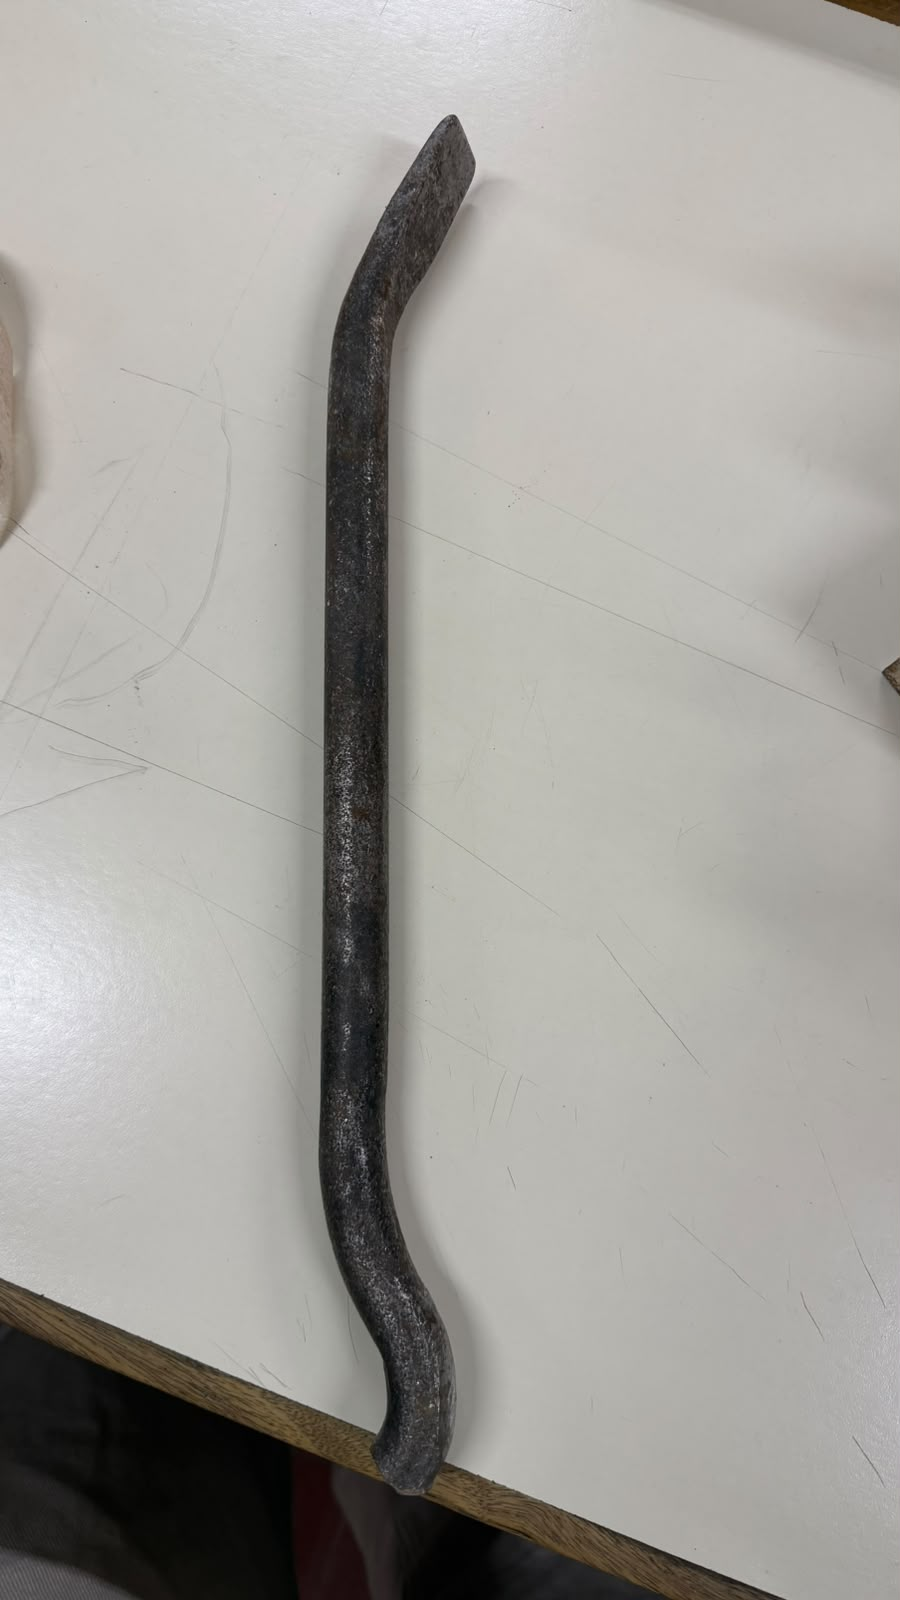
\includegraphics[height=6.5cm]{foto1.jpg}\\
\small (a) Foto 1: vista general de perfil.
\end{minipage}
\hfill
\begin{minipage}[b]{0.45\textwidth}
\centering
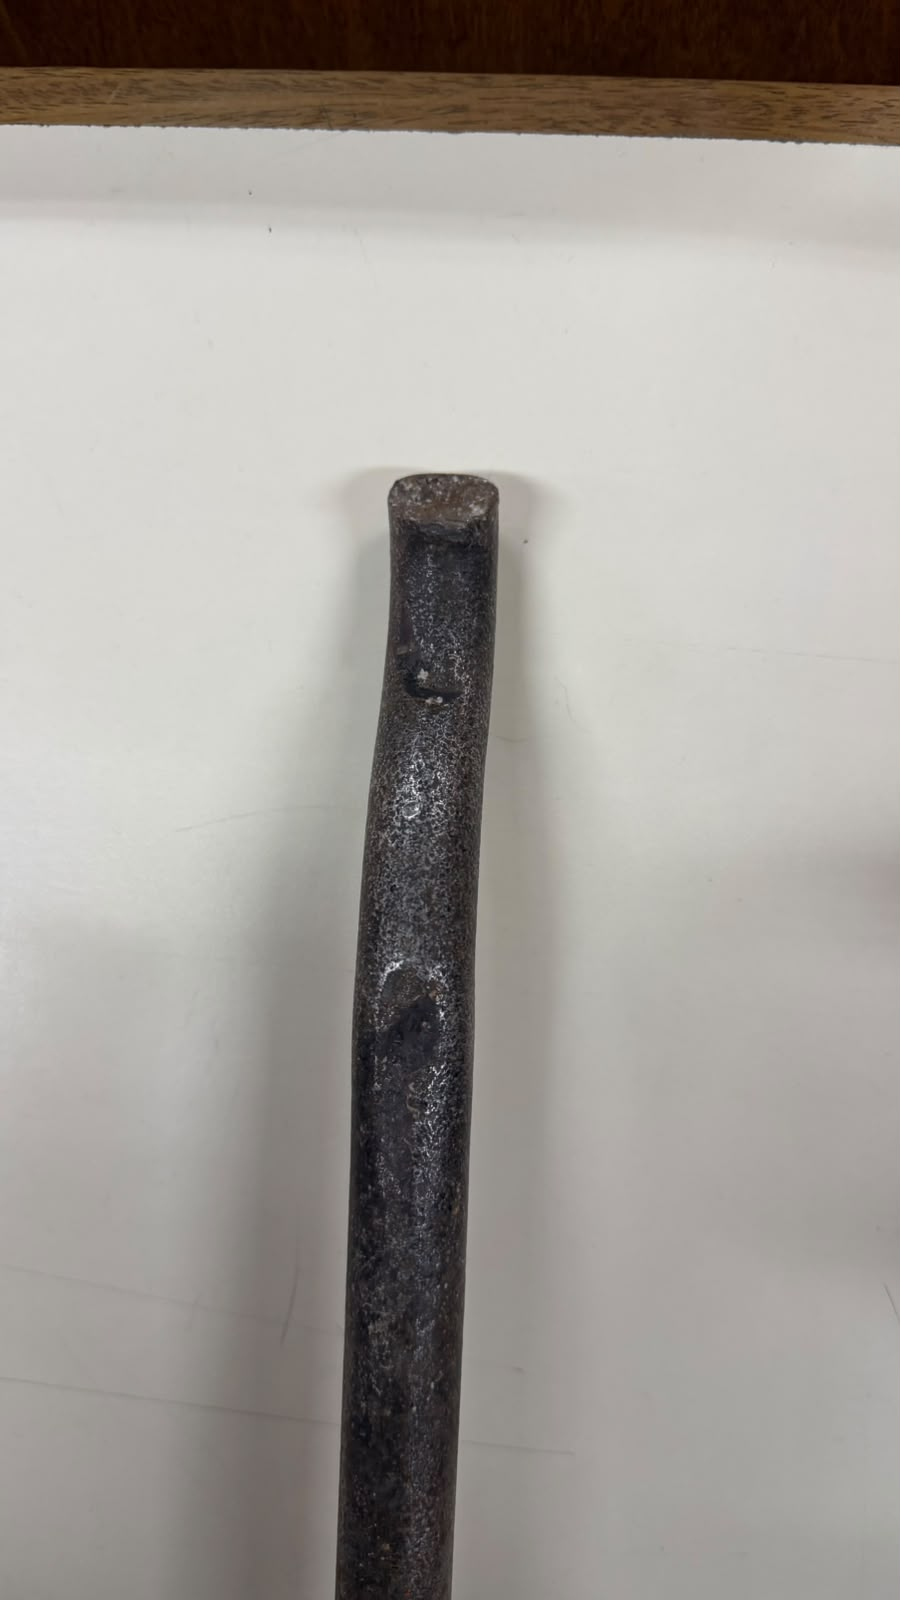
\includegraphics[height=6.5cm]{foto2.jpg}\\
\small (b) Foto 2: detalle del extremo superior.
\end{minipage}
\caption{Evidencias macroscópicas de sobrecarga en la palanqueta.}
\label{fig:general}
\end{figure}

\begin{figure}
\centering
\begin{minipage}[b]{0.31\textwidth}
\centering
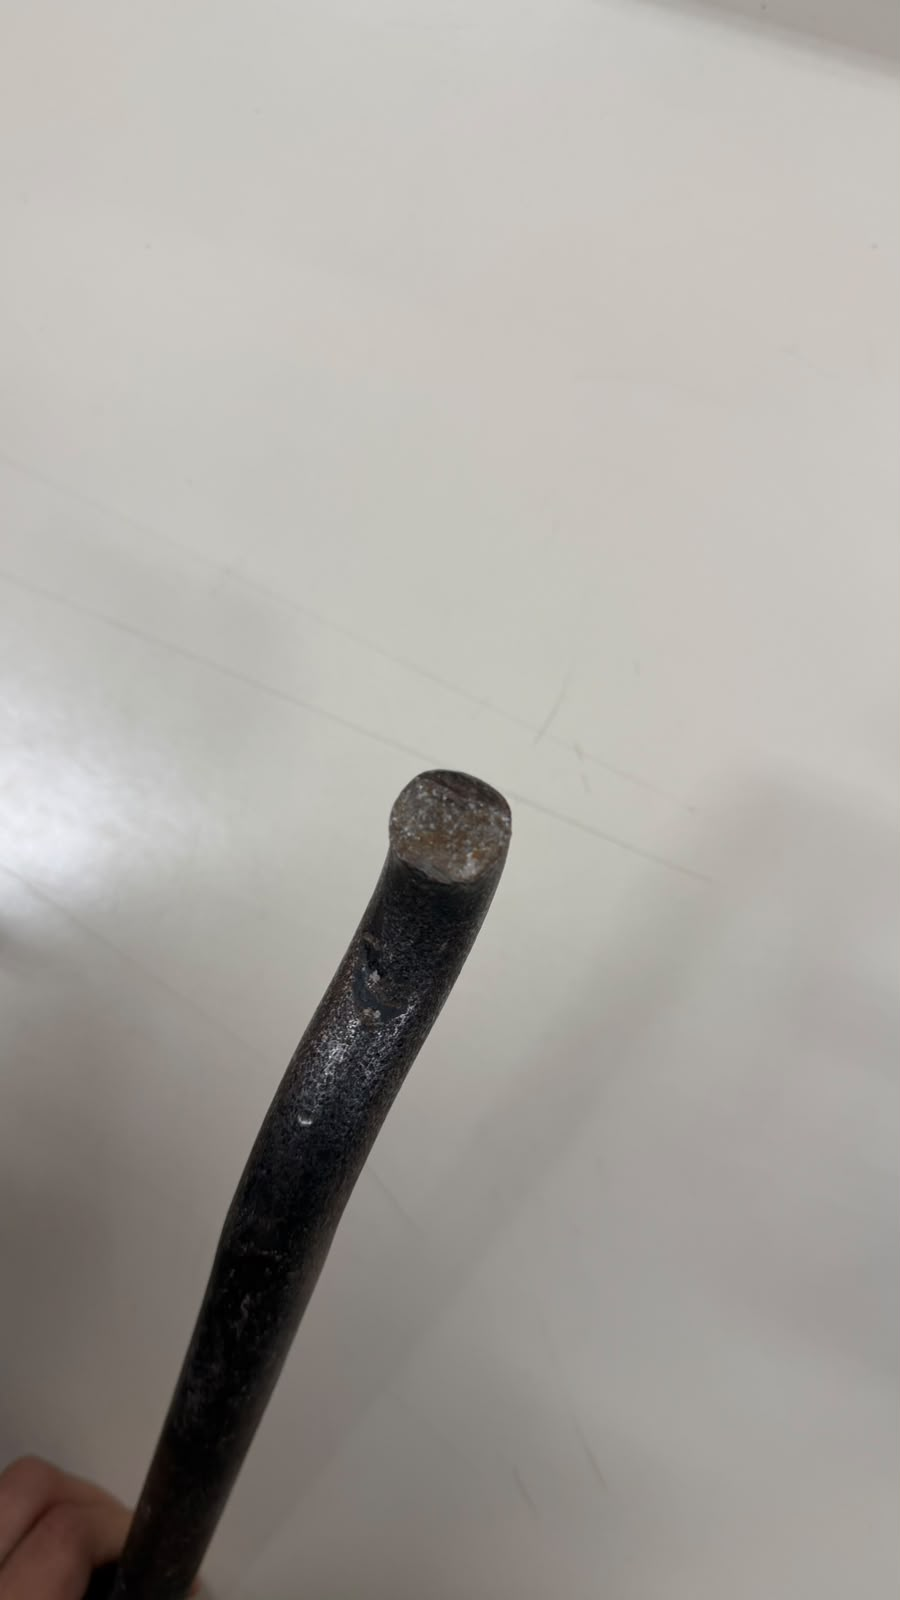
\includegraphics[height=5.5cm]{foto3.jpg}\\
\small (a) Foto 3: sección transversal superior.
\end{minipage}
\hfill
\begin{minipage}[b]{0.31\textwidth}
\centering
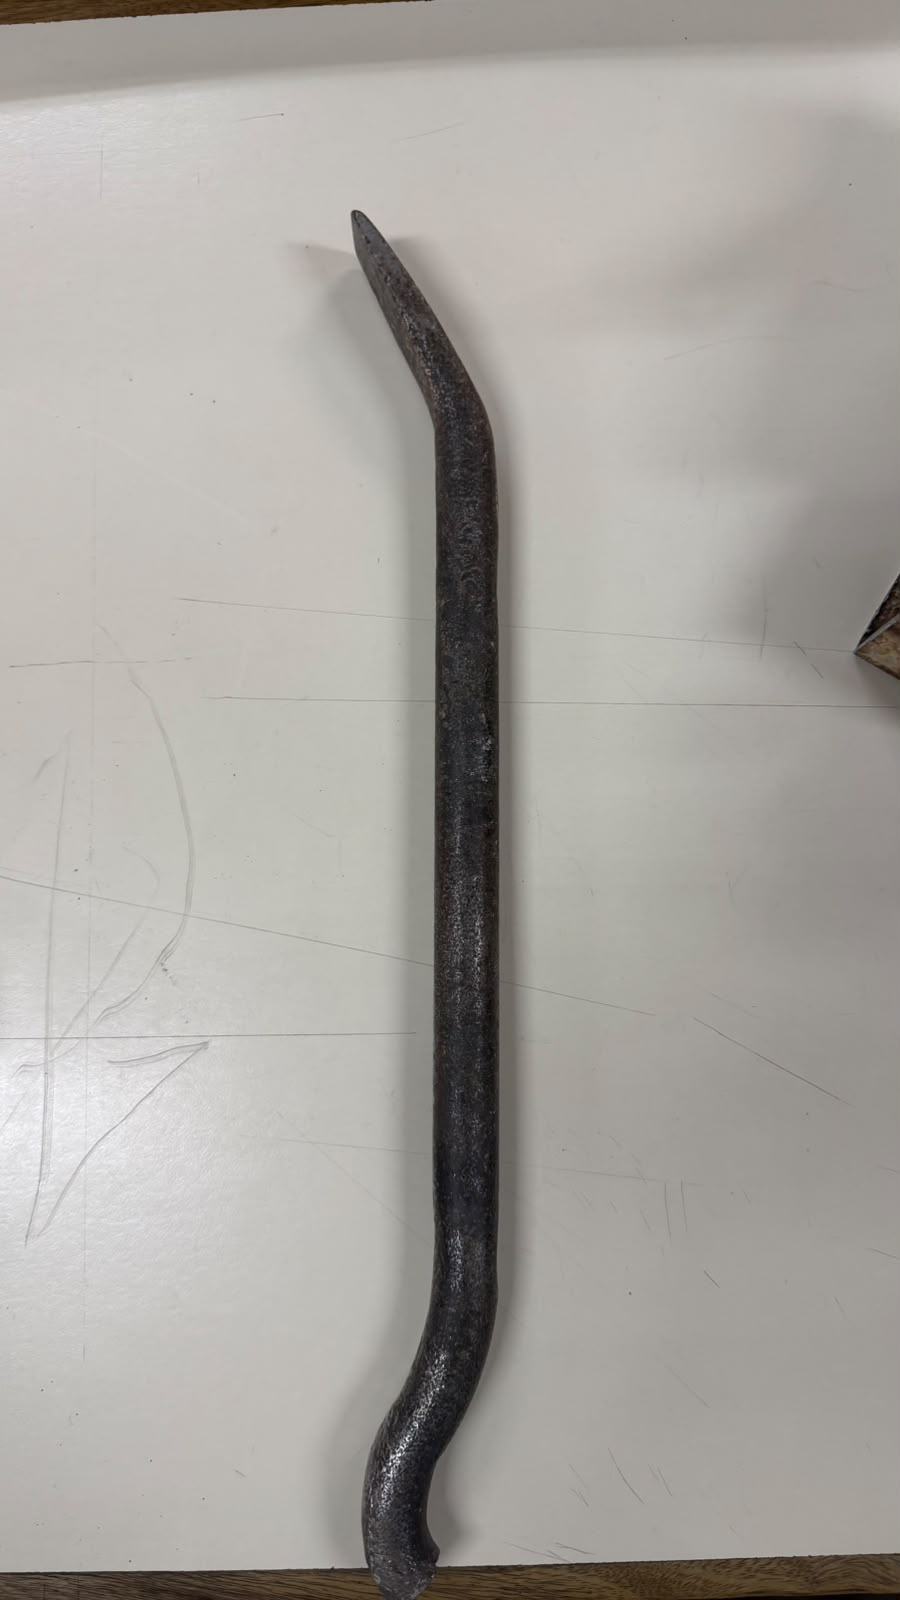
\includegraphics[height=5.5cm]{foto4.jpg}\\
\small (b) Foto 4: vista longitudinal completa.
\end{minipage}
\hfill
\begin{minipage}[b]{0.31\textwidth}
\centering
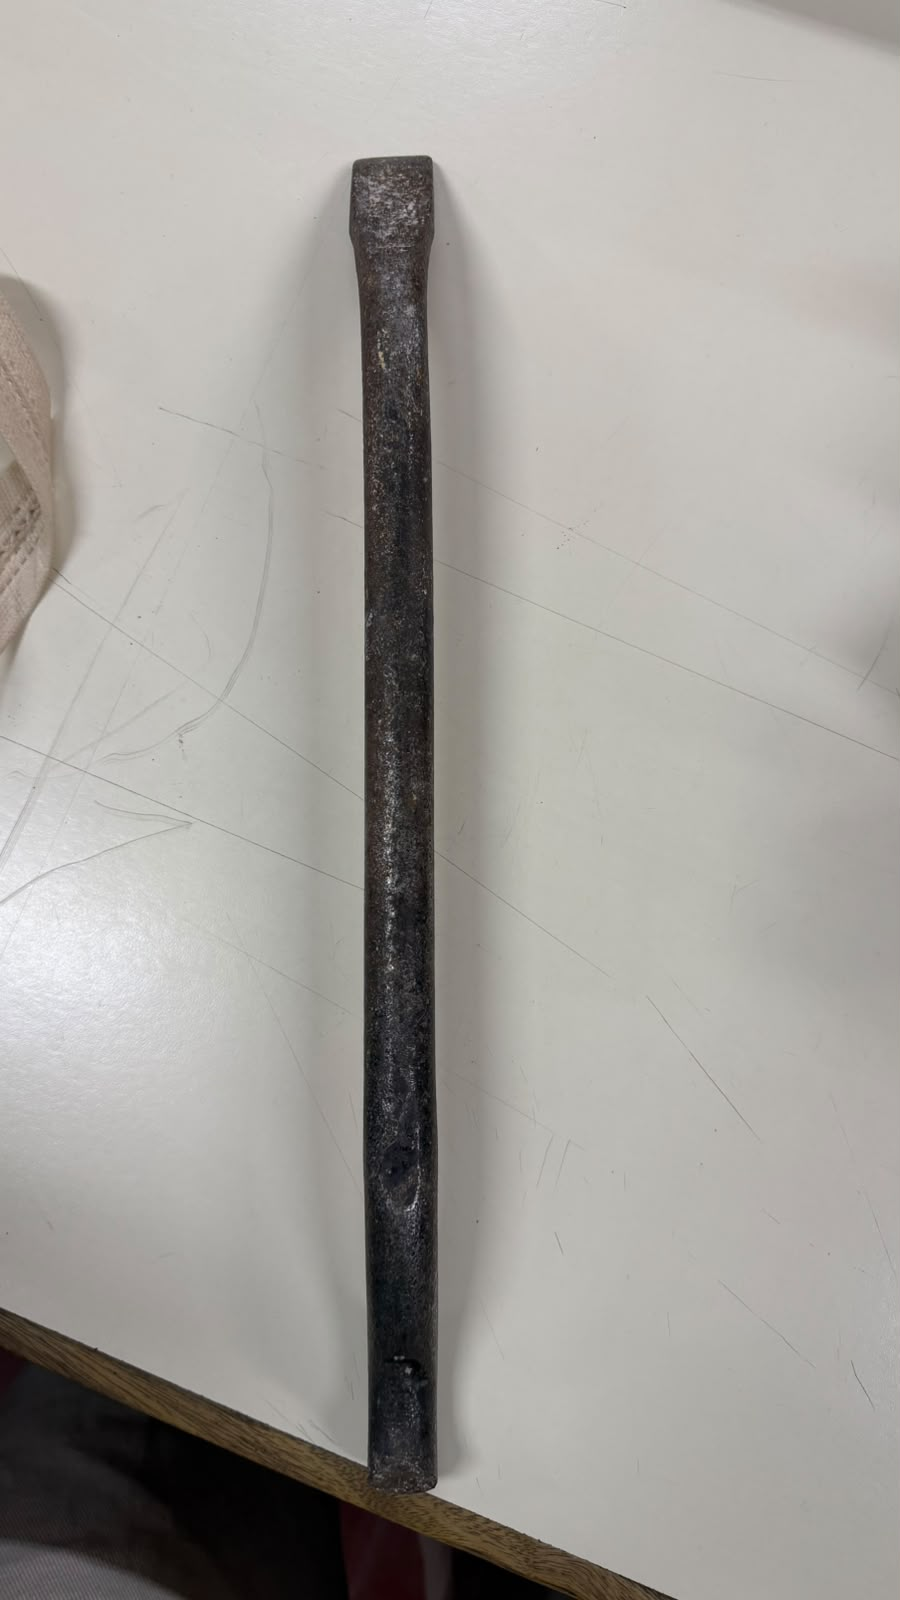
\includegraphics[height=5.5cm]{foto5.jpg}\\
\small (c) Foto 5: vista posterior y alineación del eje.
\end{minipage}
\caption{Secuencia fotográfica forense complementaria.}
\label{fig:detalle}
\end{figure}

\section{Limitaciones y recomendaciones}\label{sec:limitaciones}

El análisis fue exclusivamente visual y macroscópico, por lo que sus conclusiones son preliminares. Para un peritaje completo se recomienda:

\subsubsection{Mejoras al protocolo fotográfico.}
\begin{itemize}
\item Incluir siempre un testigo métrico (regla o escala forense) en cada toma, para medir longitud, diámetro y flecha de la curvatura.
\item Agregar un rótulo de identificación en cuadro (número de caso, fecha, pieza).
\item Utilizar iluminación controlada y rasante para resaltar relieves, marcas y texturas.
\item Mantener la cámara perpendicular a la pieza para evitar distorsión de perspectiva.
\item Conservar los archivos originales con sus metadatos (fecha, hora, equipo) sin editar.
\end{itemize}

\subsubsection{Ensayos complementarios.}
\begin{itemize}
\item Medición dimensional: longitud total, diámetro y flecha máxima de la curva.
\item Ensayo de dureza (Rockwell o Brinell) para estimar la resistencia del acero.
\item Análisis químico o metalográfico para confirmar el tipo de acero y su tratamiento térmico.
\item Inspección con lupa o microscopio de las marcas de impacto y zonas de óxido.
\end{itemize}

\subsubsection{Recomendaciones de uso.}
\begin{itemize}
\item No alargar el brazo de palanca con caños o extensiones.
\item Elegir una barra de sección adecuada a la carga a vencer.
\item No utilizarla como elemento de golpe.
\item Retirar de servicio toda barra deformada, ya que su resistencia y comportamiento son impredecibles.
\end{itemize}

\section{Conclusiones}

\textbf{Sobre la pieza.} La palanqueta falló por \emph{sobrecarga mecánica estática de flexión}. Se le aplicó un momento flector que superó el límite de fluencia del acero, lo que provocó una deformación plástica permanente. No hay evidencia de fatiga, de defectos de fabricación ni de fractura frágil, y la oxidación es superficial y secundaria.

\textbf{Sobre el comportamiento del material.} Que la barra se haya doblado sin romperse confirma que el acero es dúctil: absorbió la sobrecarga deformándose en lugar de fracturarse. Esto es deseable en una herramienta de mano, porque anticipa la falla antes de un colapso brusco.

\textbf{Sobre la causa raíz.} El origen del problema no está en el material sino en el \emph{uso inadecuado}: cargas excesivas, posible extensión del brazo de palanca y uso como elemento de impacto.

\textbf{Sobre la fotografía forense.} El taller demostró que un registro fotográfico ordenado, de lo general a lo particular, permite reconstruir el historial de esfuerzos de una pieza sin destruirla. Las fotografías fueron la base de cada conclusión y permiten que cualquier lector las verifique. La principal mejora para futuros trabajos es incorporar escala métrica y rótulo de identificación en cada toma, para pasar de un análisis cualitativo a uno cuantitativo.

\textbf{Aplicación a la ingeniería.} Este mismo método se aplica en mantenimiento y control de calidad industrial: documentar antes de intervenir, identificar el mecanismo de falla y corregir la causa raíz para que no se repita.

\begin{thebibliography}{8}

\bibitem{asm11}
ASM International: ASM Handbook, Vol.~11: Failure Analysis and Prevention. ASM International, Materials Park (2002)

\bibitem{astm860}
ASTM International: ASTM E860, Standard Practice for Examining and Preparing Items That Are or May Become Involved in Litigation. ASTM International, West Conshohocken

\bibitem{beer}
Beer, F.P., Johnston, E.R., DeWolf, J.T., Mazurek, D.F.: Mecánica de materiales, 8.ª edn. McGraw-Hill, México (2021)

\bibitem{callister}
Callister, W.D., Rethwisch, D.G.: Ciencia e ingeniería de materiales, 10.ª edn. Reverté, Barcelona (2019)

\end{thebibliography}

\end{document}
